

\tikzset{every picture/.style={line width=0.75pt}} %set default line width to 0.75pt        

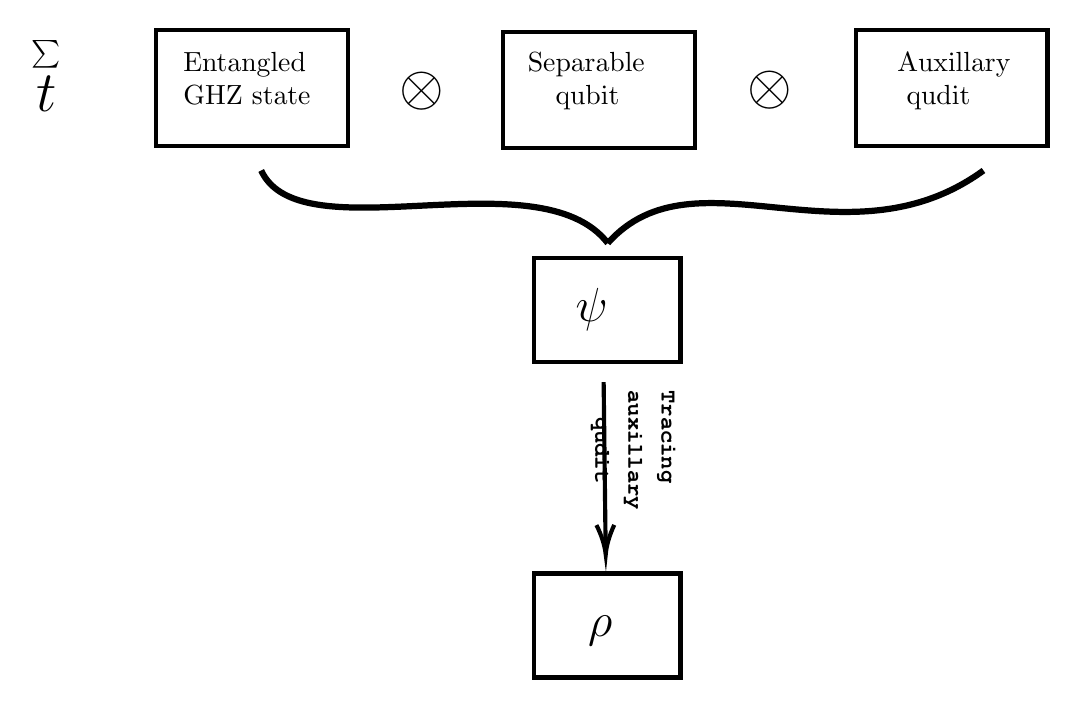
\begin{tikzpicture}[x=0.75pt,y=0.75pt,yscale=-1,xscale=1]
%uncomment if require: \path (0,418); %set diagram left start at 0, and has height of 418

%Shape: Rectangle [id:dp7294540182578855] 
\draw  [color={rgb, 255:red, 0; green, 0; blue, 0 }  ,draw opacity=1 ][fill={rgb, 255:red, 255; green, 255; blue, 255 }  ,fill opacity=1 ][line width=1.5]  (86.44,31.57) -- (178.88,31.57) -- (178.88,87.63) -- (86.44,87.63) -- cycle ;
%Shape: Rectangle [id:dp4761246648053713] 
\draw  [color={rgb, 255:red, 0; green, 0; blue, 0 }  ,draw opacity=1 ][fill={rgb, 255:red, 255; green, 255; blue, 255 }  ,fill opacity=1 ][line width=1.5]  (253.44,32.57) -- (345.88,32.57) -- (345.88,88.63) -- (253.44,88.63) -- cycle ;
%Shape: Rectangle [id:dp5375732459667567] 
\draw  [color={rgb, 255:red, 0; green, 0; blue, 0 }  ,draw opacity=1 ][fill={rgb, 255:red, 255; green, 255; blue, 255 }  ,fill opacity=1 ][line width=1.5]  (423.44,31.57) -- (515.88,31.57) -- (515.88,87.63) -- (423.44,87.63) -- cycle ;
%Shape: Rectangle [id:dp8708856606447273] 
\draw  [color={rgb, 255:red, 0; green, 0; blue, 0 }  ,draw opacity=1 ][fill={rgb, 255:red, 255; green, 255; blue, 255 }  ,fill opacity=1 ][line width=1.5]  (268.44,141.57) -- (339,141.57) -- (339,191.62) -- (268.44,191.62) -- cycle ;
%Curve Lines [id:da5387806644578281] 
\draw [line width=2.25]    (137,99.38) .. controls (156,140.38) and (271,91.77) .. (304,134.38) ;
%Curve Lines [id:da3604580216133906] 
\draw [line width=2.25]    (304,134.38) .. controls (346,87.38) and (419,147.38) .. (485,99.38) ;
%Straight Lines [id:da04531485758321774] 
\draw [line width=1.5]    (302,201.38) -- (302.96,281.38) ;
\draw [shift={(303,284.38)}, rotate = 269.31] [color={rgb, 255:red, 0; green, 0; blue, 0 }  ][line width=1.5]    (14.21,-4.28) .. controls (9.04,-1.82) and (4.3,-0.39) .. (0,0) .. controls (4.3,0.39) and (9.04,1.82) .. (14.21,4.28)   ;
%Shape: Rectangle [id:dp4350486178723396] 
\draw  [color={rgb, 255:red, 0; green, 0; blue, 0 }  ,draw opacity=1 ][fill={rgb, 255:red, 255; green, 255; blue, 255 }  ,fill opacity=1 ][line width=1.5]  (268.44,293.57) -- (339,293.57) -- (339,343.62) -- (268.44,343.62) -- cycle ;

% Text Node
\draw (97.98,41) node [anchor=north west][inner sep=0.75pt]   [align=left] {Entangled\\GHZ state};
% Text Node
\draw (263.98,41) node [anchor=north west][inner sep=0.75pt]   [align=left] {Separable\\ \ \ \ qubit};
% Text Node
\draw (441.98,41) node [anchor=north west][inner sep=0.75pt]   [align=left] {Auxillary \\ \ qudit};
% Text Node
\draw (287,154.4) node [anchor=north west][inner sep=0.75pt]  [font=\LARGE]  {$\ket{\psi }$};
% Text Node
\draw (202,50.4) node [anchor=north west][inner sep=0.75pt]  [font=\huge]  {$\mathlarger{\otimes} $};
% Text Node
\draw (370,50) node [anchor=north west][inner sep=0.75pt]  [font=\huge]  {$\mathbf{\otimes} $};
% Text Node
\draw (293,312.4) node [anchor=north west][inner sep=0.75pt]  [font=\LARGE]  {$\rho $};
% Text Node
\draw (338.5,203.88) node [anchor=north west][inner sep=0.75pt]  [rotate=-90] [align=left] {{\footnotesize {\fontfamily{pcr}\selectfont  \textbf{Tracing} }}\\{\footnotesize {\fontfamily{pcr}\selectfont \textbf{auxillary}}}\\{\footnotesize {\fontfamily{pcr}\selectfont  \ \ \textbf{qudit}}}};
% Text Node
\draw (25,35.4) node [anchor=north west][inner sep=0.75pt]  [font=\Huge]  {$\sum \limits_{{t}}$};


\end{tikzpicture}
